%%%%%%%%%%%%%%%%%%%%%%%%%%%%%%%%%%%%%%%%%%%%%%%%%%%%%%%%%%%%%%%%%%
%%%%%%%%%%%%%%%%%%%%%%%%%%%%%%%%%%%%%%%%%%%%%%%%%%%%%%%%%%%%%%%%%%
%Packages
\documentclass[10pt, a4paper]{article}
\usepackage[top=3cm, bottom=4cm, left=3.5cm, right=3.5cm]{geometry}
\usepackage{amsmath,amsthm,amsfonts,amssymb,amscd, fancyhdr, color, comment, graphicx, environ}
\usepackage{float}
\usepackage{mathrsfs}
\usepackage[math-style=ISO]{unicode-math}
% \setmathfont{TeX Gyre Termes Math}
\usepackage{lastpage}
\usepackage[dvipsnames]{xcolor}
\usepackage[framemethod=TikZ]{mdframed}
\usepackage{enumerate}
\usepackage[shortlabels]{enumitem}
\usepackage{fancyhdr}
\usepackage{indentfirst}
\usepackage{listings}
\usepackage{sectsty}
\usepackage{thmtools}
\usepackage{shadethm}
\usepackage{hyperref}
\usepackage{setspace}
\hypersetup{
    colorlinks=true,
    linkcolor=blue,
    filecolor=magenta,      
    urlcolor=blue,
}
%%%%%%%%%%%%%%%%%%%%%%%%%%%%%%%%%%%%%%%%%%%%%%%%%%%%%%%%%%%%%%%%%%
%%%%%%%%%%%%%%%%%%%%%%%%%%%%%%%%%%%%%%%%%%%%%%%%%%%%%%%%%%%%%%%%%%
%Environment setup
\mdfsetup{skipabove=\topskip,skipbelow=\topskip}
\newrobustcmd\ExampleText{%
An \textit{inhomogeneous linear} differential equation has the form
\begin{align}
L[v ] = f,
\end{align}
where $L$ is a linear differential operator, $v$ is the dependent
variable, and $f$ is a given non−zero function of the independent
variables alone.
}
\mdfdefinestyle{theoremstyle}{%
linecolor=black,linewidth=1pt,%
frametitlerule=true,%
frametitlebackgroundcolor=gray!20,
innertopmargin=\topskip,
}
\mdtheorem[style=theoremstyle]{Problem}{Problem}
\newenvironment{Solution}{\textbf{Solution.}}

\definecolor{codegreen}{rgb}{0,0.6,0}
\definecolor{codegray}{rgb}{0.5,0.5,0.5}
\definecolor{codepurple}{rgb}{0.58,0,0.82}
\definecolor{backcolour}{rgb}{0.95,0.95,0.92}

\lstdefinestyle{mystyle}{
    backgroundcolor=\color{backcolour},   
    commentstyle=\color{codegreen},
    keywordstyle=\color{magenta},
    numberstyle=\tiny\color{codegray},
    stringstyle=\color{codepurple},
    basicstyle=\ttfamily\footnotesize,
    breakatwhitespace=false,         
    breaklines=true,                 
    captionpos=b,                    
    keepspaces=true,                 
    numbers=left,                    
    numbersep=5pt,                  
    showspaces=false,                
    showstringspaces=false,
    showtabs=false,                  
    tabsize=2
}

\lstset{style=mystyle}
%%%%%%%%%%%%%%%%%%%%%%%%%%%%%%%%%%%%%%%%%%%%%%%%%%%%%%%%%%%%%%%%%%
%%%%%%%%%%%%%%%%%%%%%%%%%%%%%%%%%%%%%%%%%%%%%%%%%%%%%%%%%%%%%%%%%%
%Fill in the appropriate information below
\newcommand{\norm}[1]{\left\lVert#1\right\rVert}     
\newcommand\course{CS550 Machine Learning}                            % <-- course name   
\newcommand\hwnumber{ 5}                                 % <-- homework number
\newcommand\Information{Karan Sunil Kumbhar }                        % <-- personal information
\newcommand\Informatio{Id. - 12140860}
\newcommand\Informati{BTech CSE}
\newcommand\Informat{2025}
%%%%%%%%%%%%%%%%%%%%%%%%%%%%%%%%%%%%%%%%%%%%%%%%%%%%%%%%%%%%%%%%%%
%%%%%%%%%%%%%%%%%%%%%%%%%%%%%%%%%%%%%%%%%%%%%%%%%%%%%%%%%%%%%%%%%%
%Page setup
\pagestyle{fancy}
\headheight 35pt
\lhead{\today}
\rhead{
\includegraphics[width=1.5cm]{iitbh.png}}
\lfoot{}
\pagenumbering{arabic}
\cfoot{\small\thepage}
\rfoot{}
\headsep 1.2em
\renewcommand{\baselinestretch}{1.25}
%%%%%%%%%%%%%%%%%%%%%%%%%%%%%%%%%%%%%%%%%%%%%%%%%%%%%%%%%%%%%%%%%%
%%%%%%%%%%%%%%%%%%%%%%%%%%%%%%%%%%%%%%%%%%%%%%%%%%%%%%%%%%%%%%%%%%
%Add new commands here
\renewcommand{\labelenumi}{\alph{enumi})}
\newcommand{\Z}{\mathbb Z}
\newcommand{\R}{\mathbb R}
\newcommand{\Q}{\mathbb Q}
\newcommand{\NN}{\mathbb N}
\newcommand{\PP}{\mathbb P}
\DeclareMathOperator{\Mod}{Mod} 
\renewcommand\lstlistingname{Algorithm}
\renewcommand\lstlistlistingname{Algorithms}
\def\lstlistingautorefname{Alg.}
\newtheorem*{theorem}{Theorem}
\newtheorem*{lemma}{Lemma}
\newtheorem{case}{Case}
\newcommand{\assign}{:=}
\newcommand{\infixiff}{\text{ iff }}
\newcommand{\nobracket}{}
\newcommand{\backassign}{=:}
\newcommand{\tmmathbf}[1]{\ensuremath{\boldsymbol{#1}}}
\newcommand{\tmop}[1]{\ensuremath{\operatorname{#1}}}
\newcommand{\tmtextbf}[1]{\text{{\bfseries{#1}}}}
\newcommand{\tmtextit}[1]{\text{{\itshape{#1}}}}

\newenvironment{itemizedot}{\begin{itemize} \renewcommand{\labelitemi}{$\bullet$}\renewcommand{\labelitemii}{$\bullet$}\renewcommand{\labelitemiii}{$\bullet$}\renewcommand{\labelitemiv}{$\bullet$}}{\end{itemize}}
\catcode`\<=\active \def<{
\fontencoding{T1}\selectfont\symbol{60}\fontencoding{\encodingdefault}}
\catcode`\>=\active \def>{
\fontencoding{T1}\selectfont\symbol{62}\fontencoding{\encodingdefault}}
\catcode`\<=\active \def<{
\fontencoding{T1}\selectfont\symbol{60}\fontencoding{\encodingdefault}}

%%%%%%%%%%%%%%%%%%%%%%%%%%%%%%%%%%%%%%%%%%%%%%%%%%%%%%%%%%%%%%%%%%
%%%%%%%%%%%%%%%%%%%%%%%%%%%%%%%%%%%%%%%%%%%%%%%%%%%%%%%%%%%%%%%%%%
%Begin now!



\begin{document}

\begin{titlepage}
    \begin{center}
        \vspace*{3cm}

        \Huge
        \textbf{Machine Learning}

        \vspace{1cm}
        \huge
        Homework\hwnumber

        \vspace{1.5cm}
        \Large

        \textbf{\Information}\\                      % <-- author
        \textbf{\Informatio}\\
        \textbf{\Informati} \\
        \textbf{\Informat} \\

        \vfill

        \course \

        \vspace{1cm}

        
\includegraphics[width=0.4\textwidth]{iitbh.png}
        \\

        \Large

        \today

    \end{center}
\end{titlepage}


%%%%%%%%%%%%%%%%%%%%%%%%%%%%%%%%%%%%%%%%%%%%%%%%%%%%%%%%%%%%%%%%%%
%%%%%%%%%%%%%%%%%%%%%%%%%%%%%%%%%%%%%%%%%%%%%%%%%%%%%%%%%%%%%%%%%%
%Start the assignment now
%%%%%%%%%%%%%%%%%%%%%%%%%%%%%%%%%%%%%%%%%%%%%%%%%%%%%%%%%%%%%%%%%%
%New problem
\newpage
\subsubsection*{}

\begin{Problem}
    Suppose images are 224x224x3 and we use 64 convolutional filters that are 3x3.
    \begin{enumerate}[label=\textbf{(\alph*)}]
        \item How many responses will be computed for this layer of a CNN (stride=1, no padding)?
        \item How much zero padding is necessary to produce an output of size equal to the input?
        \item Repeat `a' for the case when the stride is 3.
    \end{enumerate}
\end{Problem}

\begin{Solution}
    \begin{enumerate}[label=\textbf{(\alph*)}]
        \item
              To calculate the number of responses (feature maps) produced by a convolutional layer in a CNN, we use the formula:

              \[
                  \text{Number of Responses} = \left(\frac{{\text{Input Size} - \text{Filter Size}}}{{\text{Stride}}} + 1\right)^2 \times \text{Number of Filters}
              \]

              Given the information:
              \begin{align*}
                  \text{Input Size}        & : 224 \times 224 \times 3 \text{ (width, height, channels)} \\
                  \text{Filter Size}       & : 3 \times 3                                                \\
                  \text{Stride}            & : 1                                                         \\
                  \text{Number of Filters} & : 64                                                        \\
              \end{align*}

              Substitute these values into the formula:
              \begin{align*}
                  \text{Number of Responses} & = \left(\frac{{224 - 3}}{{1}} + 1\right)^2 \times 64 \\
                                             & = 222 \times 222 \times 64                           \\
                                             & = 49284 \times 64                                    \\
                                             & = 3,154,176                                          \\
              \end{align*}

              Therefore, the number of responses (feature maps) computed for this layer of the CNN is $3,154,176$.
              \pagebreak
        \item
              To determine the zero padding necessary to produce an output of the same
              size as the input, we use the formula:

              \[ \text{Output Size} = \frac{\text{Input Size} - \text{Filter Size} + 2
                      \times \text{Padding}}{\text{Stride}} + 1 \]

              Given the information: \begin{align*} \text{Input Size} & : 224 \times 224
               \text{ (width, height)}              \\ \text{Filter Size} & : 3 \times 3 \\
               \text{Stride}     & : 1              \\ \text{Output Size} & : 224 \times 224\end{align*}

              Substitute these values into the formula and solve for Padding:
              \begin{align*}
                  224 & = \frac{224 - 3 + 2 \times \text{Padding}}{1} + 1 \\
                  224 & = 221 + 2 \times \text{Padding} +1
              \end{align*}
              Solving for Padding:
              \begin{align*}
                  2 \times \text{Padding} & = 224 - 221 - 1 \\
                  2 \times \text{Padding} & = 2             \\
                  \text{Padding}          & = \frac{2}{2}   \\
                                          & = 1
              \end{align*}

              Therefore, the necessary zero padding to produce an output of the same size
              as the input is \textbf{$1$ in each dimension.}
              \pagebreak
        \item
              To calculate the number of responses when the stride is 3, we use the formula:

              \[
                  \text{Number of Responses} = \left(\frac{\text{Input Size} - \text{Filter Size}}{\text{Stride}} + 1\right)^2 \times \text{Number of Filters}
              \]

              Given the information:
              \begin{align*}
                  \text{Input Size}        & : 224 \times 224 \text{ (width, height)} \\
                  \text{Filter Size}       & : 3 \times 3                             \\
                  \text{Stride}            & : 3                                      \\
                  \text{Number of Filters} & : 64                                     \\
              \end{align*}

              Substitute these values into the formula:
              \begin{align*}
                  \text{Number of Responses} & = \left(\frac{224 - 3}{3} + 1\right)^2 \times 64 \\
                                             & = \left(73.67+1\right) \times 64
              \end{align*}
              here we can see dimension is fractional so here we can do 2 thing eighter discard last 2 columns and 2 rows or another way add proper padding
              \begin{itemize}
                  \item discarding extra dimension(taking $73.67 \approx 73$), we get
                        \begin{align*}
                            \text{Number of Responses} & = \left(73+1\right) \times 64 \\
                                                       & = 74 \times 74 \times 64      \\
                                                       & = 5476 \times 64              \\
                                                       & = 350464
                        \end{align*}
                  \item Adding proper padding (taking $73.67 \approx 74$), we get
                        \begin{align*}
                            \text{Number of Responses} & = \left(74+1\right) \times 64 \\
                                                       & = 75 \times 75 \times 64      \\
                                                       & = 5625 \times 64              \\
                                                       & = 360000
                        \end{align*}
              \end{itemize}
              Therefore, the number of responses computed for this layer of the CNN with a stride of 3 is
              $350,464$(when discard extra dimensions) or $360000$ (adding proper padding).

    \end{enumerate}


\end{Solution}

%%%%%%%%%%%%%%%%%%%%%%%%%%%%%%%%%%%%%%%%%%%%%%%%%%%%%%%%%%%%%%%%%%
%New problem
\newpage
\subsubsection*{}
\begin{Problem}
    Assume that the inputs are single bits 0 (white) and 1 (black). Consider a 3x3
    filter, whose weights are \(w_{ij}\), for \(0 \leq i \leq 2\) and \(0 \leq j \leq 2\) and whose bias
    is b. Suggest weights and bias so that the output of this filter will detect the
    following simple features.
    \begin{enumerate}[label=\textbf{(\alph*)}]
        \item Vertical boundary, where the left column is 0, and the other two columns are 1.
        \item A diagonal boundary, where only the triangle of three pixels in the upper right corner are 1
        \item A corner, in which the 2x2 square in the lower right is 0 and the other pixels \\ are 1.
    \end{enumerate}
\end{Problem}

\begin{Solution}
    \begin{enumerate}[label=\textbf{(\alph*)}]
        \item
              To detect a vertical boundary where the left column is 0
              and the other two columns are 1, we can use the following filter:

              \[ \text{Weight Matrix:} \quad \begin{bmatrix} 0 & 1 & 1 \\ 0 & 1
                  & 1     \\ 0 & 1 & 1 \\\end{bmatrix} \]

              \[ \text{Bias:} \quad -5 \]

              When this filter is applied to an input matrix representing the
              pattern, it should produce a high value(in this case high value
              is 6), indicating the detection of the vertical boundary. For all
              other pattern it will produce less value than 6. And when we add bias -5
              to it will give value as 1 or less than 1. And then we will apply Relu
              activation function to get desired output(pixel value 1 correspoding to
              required pattern and others values are zeros).
        \item
              To detect a diagonal boundary where only the triangle of three
              pixels in the upper right corner is 1, we can use the following filter:

              \[ \text{Weight Matrix:} \quad \begin{bmatrix} 0 & 1 & 1 \\ 0 & 0 & 1
                \\ 0 & 0 & 0 \\\end{bmatrix} \]

              \[ \text{Bias:} \quad -2 \]

              When this filter is applied to an input matrix representing the pattern,
              it should produce a high value as 3, indicating the detection of the
              diagonal boundary in the upper right corner. In all other cases it
              is less than 3. And then when we add bias term to it will product values one or less than one.
              And after applying Relu activation function it will produce one corresponding to required pattern and
              other values are zero.
        \item
              To detect a corner where the 2x2 square in the lower
              right is 0, and the other pixels are 1, you can use the following
              filter:

              \[ \text{Weight Matrix:} \quad \begin{bmatrix} 1 & 1 & 1 \\ 1 & 0
                  & 0     \\ 1 & 0 & 0 \\\end{bmatrix} \]

              \[ \text{Bias:} \quad -4 \]

              When this filter is applied to an input matrix representing the
              pattern, it should produce a high value, indicating the detection
              of the corner with highest value as 5 and after adding bias it will produce 1 or less than one.
              And then applying Relu activation function we will get 1 values corresponding to corner and zero
              correspoding to lower right square. We also can apply logical not to output after applying Relu function
              to get high values correspoding to right lower square
    \end{enumerate}
\end{Solution}

%%%%%%%%%%%%%%%%%%%%%%%%%%%%%%%%%%%%%%%%%%%%%%%%%%%%%%%%%%%%%%%%%%
%New problem
\newpage
\subsubsection*{}
\begin{Problem}
    In this exercise, you are asked to design the input weights for one or more
    nodes of the hidden state of an RNN. The input is a sequence of bits, 0 or 1
    only. Note that you can use other nodes to help with the node requested. Also
    note that you can apply a transformation to the output of the node so a ``yes''
    answer has one value and a ``no'' answer has another.
    \begin{enumerate}
        \item A node to signal when the input is 1 and the previous input is 0
        \item A node to signal when the last three inputs have all been 1
        \item A node to signal when the input is the same as the previous input
    \end{enumerate}
\end{Problem}

\begin{Solution} \newline
    \begin{enumerate}
        \item
              We can create state table as follows
              \begin{table}[ht] \centering \begin{tabular}{ccc} \textbf{ht-1} &
               \textbf{xt}         & \textbf{ht}     \\ \hline 0 & 0 & 1 \\ 1 & 0 & 0 \\ 2 & 0 & 2 \\ 0
                                   & 1           & 0 \\ 1 & 1 & 2 \\ 2 & 1 & 2 \\\end{tabular} \caption{State machine
                      table} \label{tab:state_machine} \end{table}

              The transition rule is given by:
              \[ h_{t+1} = \begin{cases} 1 & \text{if }
              x_t + h_{t-1} = 0 \\ 0 & \text{if } x_t + h_{t-1} = 1 \\ 2 & \text{if } x_t
              + h_{t-1} \geq 2  \\\end{cases} \]
        \item
              We can create state table as follows
              \begin{table}[ht] \centering \begin{tabular}{ccc} \textbf{ht-1}
                       & \textbf{xt} & \textbf{ht} \\ \hline 0 & 0 & 0 \\ 1 & 0 & 0 \\ 2 & 0 &
                      0                            \\ 3 & 0 & 3 \\ 0 & 1 & 1 \\ 1 & 1 & 2 \\ 2 & 1 & 3 \\ 3 & 1 & 3 \\
                  \end{tabular} \caption{State machine table} \label{tab:state_machine_2}
              \end{table}

              The transition rule is given by: \[ h_{t+1} = \begin{cases} 3 &
              \text{if } h_t + 1 \geq 3 \\ (h_t + 1) \cdot (x_t) & \text{if } h_t + 1
              < 3                       \\\end{cases} \]
    \end{enumerate}
\end{Solution}


%%%%%%%%%%%%%%%%%%%%%%%%%%%%%%%%%%%%%%%%%%%%%%%%%%%%%%%%%%%%%%%%%%
%New problem
\newpage
\subsubsection*{}
\begin{Problem}
    Let A be a matrix of 4-dimensional data points
    \[ \text{A =} \quad \begin{bmatrix} 1 & 1 \\ 2 & 4
                \\ 3 & 9 \\ 4 & 16\end{bmatrix} \]

    \begin{enumerate}
        \item  Compute Eigenpairs for $A^{T}A$?
        \item  What do you expect the eigenvalues of $AA^{T}$ to be?
        \item  Find the eigenvectors of $AA^{T}$, using the eigenvalues from part (c).
        \item Write the 1-dimensional and 2-dimensional encodings (z) of
              columns of $A$ using $PCA$.
              \begin{center}
                  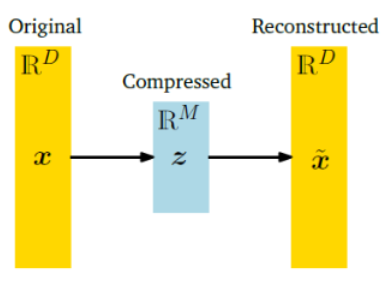
\includegraphics[width=0.4\textwidth]{images/q4.png} \\
              \end{center}
    \end{enumerate}
\end{Problem}

\begin{Solution}
    \begin{enumerate}
        \item
              To compute the eigenpairs for $A^TA$, where $A$ is a matrix of
              4-dimensional data points given by

              \[ A = \begin{bmatrix} 1 & 1 \\ 2 & 4 \\ 3 & 9 \\ 4 & 16 \end{bmatrix} \]

              we follow these steps:

              1. \textbf{Calculate $A^TA$:}
              \begin{align*}
                  A^TA & = \begin{bmatrix}
                               1 & 2 & 3 & 4  \\
                               1 & 4 & 9 & 16
                           \end{bmatrix}
                  \begin{bmatrix}
                      1 & 1  \\
                      2 & 4  \\
                      3 & 9  \\
                      4 & 16
                  \end{bmatrix}                   \\
                       & = \begin{bmatrix}
                               1+4+9+16  & 1+8+27+64   \\
                               1+8+27+64 & 1+16+81+256
                           \end{bmatrix} \\
                       & = \begin{bmatrix}
                               30  & 100 \\
                               100 & 354
                           \end{bmatrix}
              \end{align*}

              2. \textbf{Find Eigenvalues ($\lambda$):} The characteristic equation is given
              by:
              \begin{align*}
                  |A^TA - \lambda I| & = \begin{vmatrix}
                                             30-\lambda & 100         \\
                                             100        & 354-\lambda
                                         \end{vmatrix}                                     \\
                                     & = (30 - \lambda)(354 - \lambda) - 100 \times 100 \quad = 0     \\
                  0                  & = 30\times 354  + \lambda^{2} - (354+30)\times \lambda - 10000 \\
                  0                  & = \lambda^2 - 384\lambda + 620
              \end{align*}

              Solving this quadratic equation will give us the eigenvalues.


              \[ (\lambda^2 - 384\lambda + 620) = 0 \]

              This equation can be solved using the quadratic formula:

              \[ \lambda = \frac{-b \pm \sqrt{b^2 - 4ac}}{2a} \]

              where \( a = 1 \), \( b = -384 \), and \( c = 620 \).
              Substituting these values:

              \[ \lambda = \frac{384 \pm \sqrt{(-384)^2 - 4 \times 1 \times
                          620}}{2 \times 1} \]

              \[ \lambda = \frac{384 \pm \sqrt{147456 - 2480}}{2} \]

              \[ \lambda = \frac{384 \pm \sqrt{144976}}{2} \]

              \[ \lambda = \frac{384 \pm 380.75}{2} \]

              So, we have two possible solutions:

              \begin{align*}
                  \lambda_1 & = \frac{384 + 380.75}{2} \\
                            & = 382.375                \\
                  \lambda_2 & =\frac{384 - 384.75}{2}  \\
                            & = 1.625
              \end{align*}

              Given the eigenvalue equation
              \(A^TA \mathbf{v} = \lambda \mathbf{v}\) with

              \[ A^TA = \begin{bmatrix} 30 & 100 \\ 100 & 354 \end{bmatrix} \]

              the calculated eigenvalues and corresponding eigenvectors are as
              follows:

              1. For \(\lambda = 1.625\), the corresponding eigenvector is any
              non-zero multiple of \(\begin{bmatrix} 100 \\ -28.375
              \end{bmatrix}\).

              2. For \(\lambda = 382.375\), the corresponding eigenvector is
              any non-zero multiple of \(\begin{bmatrix} 100 \\ 352.375
              \end{bmatrix}\).

              Therefore, the eigenpairs are \((1.625, \begin{bmatrix} 100 \\
                  -28.375\end{bmatrix})\) and \((382.375, \begin{bmatrix} 100 \\
                  352.375\end{bmatrix})\).
        \item
              To find the eigenvalues of \(A A^T\), where \(A\) is the given
              matrix

              \[ A = \begin{bmatrix} 1 & 1 \\ 2 & 4 \\ 3 & 9 \\ 4 & 16 \end{bmatrix}
              \]

              we can use the property that the eigenvalues of \(A A^T\) are the same
              as the eigenvalues of \(A^T A\). From our previous discussion, we found
              that the eigenvalues of \(A^T A\) are \(1.625\) and \(382.375\).
              Therefore, the expected eigenvalues of \(A A^T\) are also \(1.625\) and
              \(382.375\).
        \item
              Given the matrix \(A A^T\):

              \[ A A^T = \begin{bmatrix} 2  & 6  & 12 & 20  \\ 6 & 20 & 42 & 72 \\
                12 & 42 & 90 & 156 \\ 20 & 72 & 156 & 272\end{bmatrix} \]
              \begin{itemize}
                  \item
                        For the eigenvalue \(\lambda = 1.625\), the corresponding
                        eigenvector \(\mathbf{v}\) satisfies the system of equations:
                        \begin{align*}
                            A\times a^{T} \times v  = \lambda \times v \\
                            \begin{bmatrix} 2  & 6  & 12 & 20  \\ 6 & 20 & 42 & 72 \\
                12 & 42 & 90 & 156 \\ 20 & 72 & 156 & 272\end{bmatrix}
                            \begin{bmatrix}
                                w \\
                                x \\
                                y \\
                                z \\
                            \end{bmatrix} & =
                            1.625 \times
                            \begin{bmatrix}
                                w \\
                                x \\
                                y \\
                                z \\
                            \end{bmatrix}
                        \end{align*}
                        so value of v is non-zero multiple of $\begin{bmatrix}
                                -1.32 \\
                                -1.60 \\
                                -0.82 \\
                                1
                            \end{bmatrix}$

                  \item
                        For the eigenvalue \(\lambda = 382.375\), the corresponding
                        eigenvector \(\mathbf{v}\) satisfies the system of equations:
                        \begin{align*}
                            A\times a^{T} \times v  = \lambda \times v \\
                            \begin{bmatrix} 2  & 6  & 12 & 20  \\ 6 & 20 & 42 & 72 \\
                12 & 42 & 90 & 156 \\ 20 & 72 & 156 & 272\end{bmatrix}
                            \begin{bmatrix}
                                w \\
                                x \\
                                y \\
                                z \\
                            \end{bmatrix} & =
                            382.375 \times
                            \begin{bmatrix}
                                w \\
                                x \\
                                y \\
                                z \\
                            \end{bmatrix}
                        \end{align*}
                        so value of v is non-zero multiple of $\begin{bmatrix}
                                -0.37 \\
                                0.27  \\
                                0.57  \\
                                1
                            \end{bmatrix}$
              \end{itemize}
        \item
              \begin{itemize}
                  \item
                        1-dimensional encoding (z) of columns of A using PCA = A.
                        for first value of v
                        \begin{align*}
                            A^{T}\times A =\begin{bmatrix}
                                               1   & 1  \\
                                               2   & 4  \\
                                               3   & 9  \\
                                               4 0 & 16
                                           \end{bmatrix} \times
                            \begin{bmatrix}
                                100 \\ -28.375
                            \end{bmatrix}
                             & = \begin{bmatrix}
                                     71.625 \\ 86.5 \\44.625 \\-54
                                 \end{bmatrix}
                        \end{align*}
                  \item
                        2-dimensional encoding (z) of columns of A using PCA = A.
                        eigenvectors of
                        \begin{align*}
                            A^{T}\times A & = \begin{bmatrix}
                                                  1 & 1  \\
                                                  2 & 4  \\
                                                  3 & 9  \\
                                                  4 & 16
                                              \end{bmatrix}
                            \times
                            \begin{bmatrix}
                                100     & 100     \\
                                -28.375 & 352.375
                            \end{bmatrix}                   \\
                                          & = \begin{bmatrix}
                                                  71.625 & 452.375  \\
                                                  86.5   & 1609.5   \\
                                                  44.625 & 3471.375 \\
                                                  -54    & 6038
                                              \end{bmatrix}
                        \end{align*}
              \end{itemize}

    \end{enumerate}
\end{Solution}
%%%%%%%%%%%%%%%%%%%%%%%%%%%%%%%%%%%%%%%%%%%%%%%%%%%%%%%%%%%%%%%%%%


%New problem
\newpage
\subsubsection*{}
\begin{Problem}
    Design a CNN that can detect the face in the given input image \\
    \begin{center}
        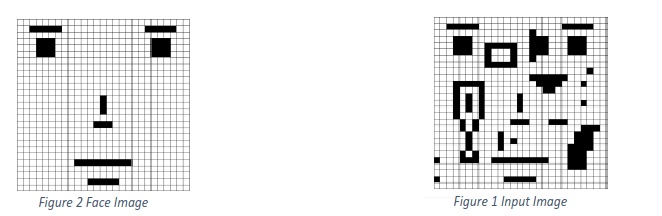
\includegraphics[width=0.7\textwidth]{images/q5.png} \\
    \end{center}
    \begin{enumerate}
        \item What strategy will you use? How many layers? How many
              filters?
        \item Describe the filters for each layer in detail.
        \item Show how the convolutions will work and demonstrate that your CNN will be able to
              detect this pattern.
    \end{enumerate}
\end{Problem}

\begin{Solution}
    \begin{enumerate}
        \item
              Strategy, Layers and Filters
              \begin{itemize}
                  \item We can create small features to detect each part of face and then we will combine this
                        features to get or detect complete face
                  \item we will mainly use 3 layers which will describe in below part solution
                  \item we will mainly taking 5 filter in first layer and then to get combine part like nose, eyes, mouth we again
                        use 3 filters. And then we can get eighter full face or partial face(here while creating filters, we are treating black part as 1 and white part as 0. And to
                        to detect part required we are putting high value correspondig to it)
              \end{itemize}
        \item Filters and Layers details
              \begin{itemize}
                  \item[\textbf{layer 1}] :-
                      \begin{itemize}
                          \item[Filter 1] : Horizontal filter(denoted by letter H)
                              \begin{center}
                                  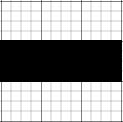
\includegraphics[width=0.1\textwidth]{images/L1-Horizontal-filter.png} \\
                              \end{center}
                              This filter will detect horizontal blocks of size $3 \times 1$ which belongs may be mouth, nose or eyes
                          \item[Filter 2] : Vertical filter(denoted by letter V)
                              \begin{center}
                                  
\includegraphics[width=0.1\textwidth]{images/L1-Vertical-filter.png} \\
                              \end{center}
                              This filter will detect Vertical blocks of size $1 \times 3$ which belongs may be nose
                              \item[Filter 3]: Block filter(denote by letter B)
                              \begin{center}
                                  
\includegraphics[width=0.1\textwidth]{images/L1-Eye-block-filter.png} \\
                              \end{center}
                              This filter will detect  blocks of size $3 \times 3$ which belongs may be eyes
                              \item[Filter 4]: Left filter(denote by letter L)
                              \begin{center}
                                  
\includegraphics[width=0.1\textwidth]{images/L1-Left-filter.png} \\
                              \end{center}
                              This filter will detect  blocks of size $1 \times 1$ which belongs may be eye part or mouth
                              \item[Filter 5]: Right filter(denote by letter R)
                              \begin{center}
                                  
\includegraphics[width=0.1\textwidth]{images/L1-Right-filter.png} \\
                              \end{center}
                              This filter will detect blocks of size $1 \times 1$ which belongs may be eye part or mouth
                      \end{itemize}
                  \item[\textbf{layer 2}] :-
                      \begin{itemize}
                          \item[Filter 1] : Nose filter(denoted by letter N)
                              \begin{center}
                                  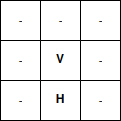
\includegraphics[width=0.1\textwidth]{images/L2-Nose-filter.png} \\
                              \end{center}
                              This filter will detect Nose part of face (combination of vertical and horizontal block which are detected in first layer)
                          \item[Filter 2] Mouth filter: (denoted by letter M)
                              \begin{center}
                                  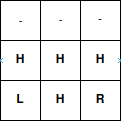
\includegraphics[width=0.1\textwidth]{images/L2-Mouth-filter.png} \\
                              \end{center}
                              This filter will detect Mouth part of face (Combination of two horizontal strips. First one is of size $1 \times 9$ which is combination of again three horizonatal filter.
                              And another below one strip is of size $1 \times 5$ which is combination of $\text{left} + \text{horizonatal} + \text{right}$ filter )

                              \item[Filter 3]: Eyes filter(denote by letter E)
                              \begin{center}
                                  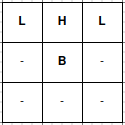
\includegraphics[width=0.1\textwidth]{images/L2-Eye-filter.png} \\
                              \end{center}
                              This filter will detect  eyes part of face(This is combination of eyebrow and block feature. Here eyebrow part is combination of $\text{left}+\text{horizontal}+\text{right}$
                              And Block is feature detected in layer 1)
                      \end{itemize}
                      \newpage
                  \item[\textbf{layer 3}] :-
                      \begin{itemize}
                          \item[Filter 1] : Full face(denoted by letter F)
                              \begin{center}
                                  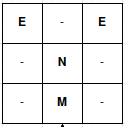
\includegraphics[width=0.1\textwidth]{images/L3-full-face.png} \\
                              \end{center}
                              This filter will detect full face (combination of two eyes, one nose and mouth)
                          \item[Filter 2] Mouth filter: (denoted by letter M)
                              \begin{center}
                                  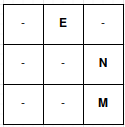
\includegraphics[width=0.1\textwidth]{images/L3-Parital-face.png} \\
                              \end{center}
                              This filter will detect partial face (Combination of of one nose, mouth and one eye)
                      \end{itemize}
              \end{itemize}
        \item Demostration
              \begin{center}
                  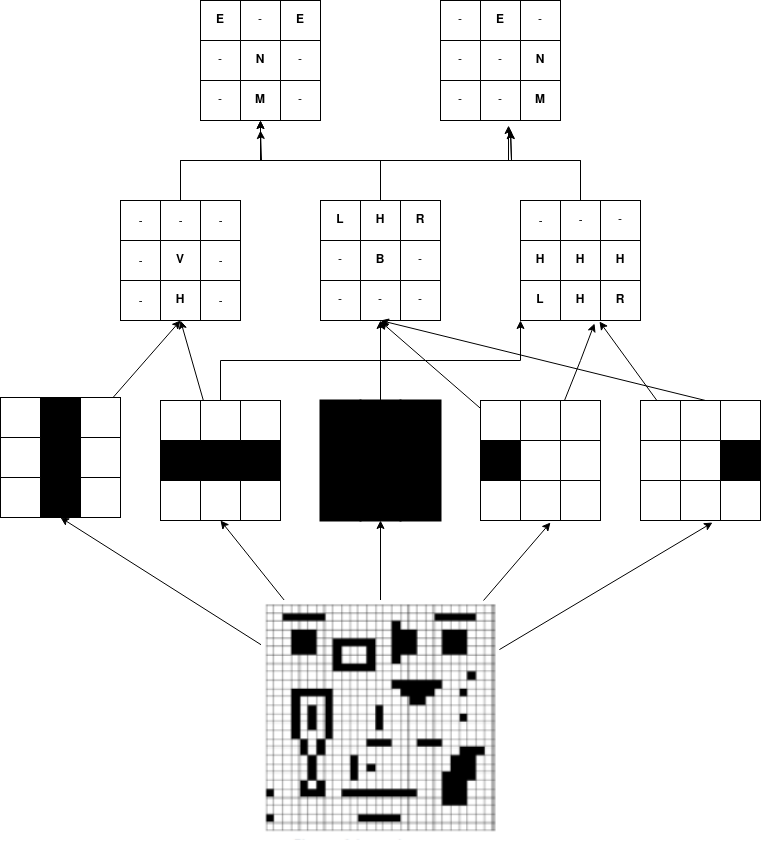
\includegraphics[width=0.8\textwidth]{images/q5_ans.png} \\
              \end{center}

    \end{enumerate}
\end{Solution}
%%%%%%%%%%%%%%%%%%%%%%%%%%%%%%%%%%%%%%%%%%%%%%%%%%%%%%%%%%%%%%%%%%
%Complete the assignment now
\end{document}

%%%%%%%%%%%%%%%%%%%%%%%%%%%%%%%%%%%%%%%%%%%%%%%%%%%%%%%%%%%%%%%%%%
%%%%%%%%%%%%%%%%%%%%%%%%%%%%%%%%%%%%%%%%%%%%%%%%%%%%%%%%%%%%%%%%%%

